\newpage
\section{Evaluation}

%% Functional Prototype %%
\subsection{Functional Prototype}

% Should talk about the hardware, software, and cloud infrastructure we used compared to what we wanted.

\subsubsection{Hardware}

For our functional prototype, we used the ESP32-C3 microcontroller, solenoid lock, LEDs, transistors, and a keypad. The ESP32-C3 is the brain of the entire lock, being able to send and recieve signals from the server. Compared to our manufactured design, we will be building our own microcontroller so that it is customized to have the required functionality we need for our lock. As for the solenoid lock, we also plan to use an industry standard lock so that it can actually work on a standard door. Our microcontroller reads and write to the server, then controls the door lock to either lock or unlock. Furthermore, when it finishes doing a task of locking or unlocking, it will send back an acknowledgement that the task is officially done. The microcontroller for our prototype uses wifi provisioning (acts as an access point) to let users fill in parameters of their wifi SSID and password, along side the API key. In our manufactured design though, we plan to use bluetooth to do all the setup instead of using wifi provisioning.

\begin{figure}[!ht]
    \centering
    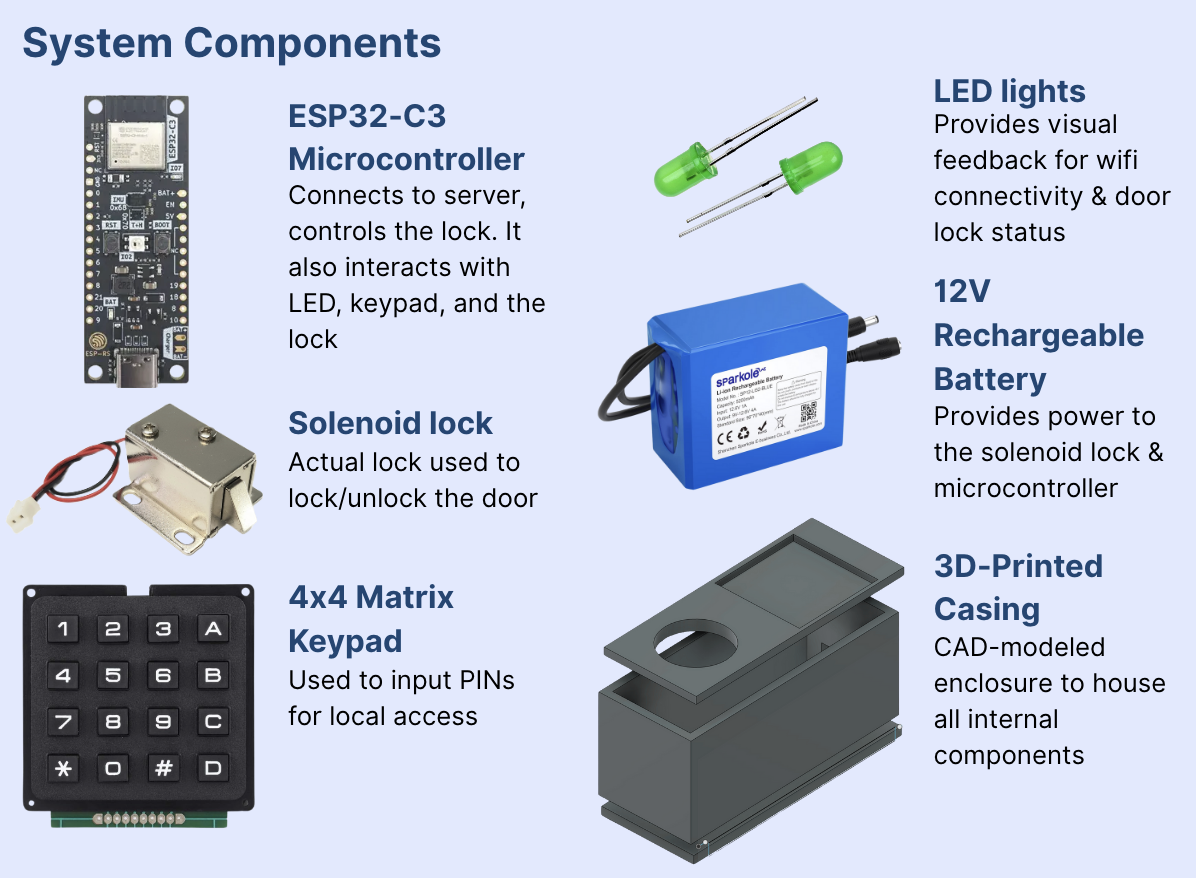
\includegraphics[width=1\textwidth]{img/hardwareComponents.png}
    \label{fig:hardwareComponents}
\end{figure}

For our hardware, we also used up 99\% of the ESP32-C3 storage. We also utilized power supplies for our functional prototype since the solenoid lock required 12V to unlock the lock. 

\subsubsection{Software}

The functional prototype of the app currently uses the Swift language. This is what we wanted especially for native IOS apps, and in our manufactured design we plan to use the same language. Though we also would like to produce the same app on other non IOS devices as well. The app currently is able to allow users to sign in and sign up, unlock and lock the door, generating one time pins, accessing emergency pins, and logging out. 

\begin{figure}[!ht]
    \centering
    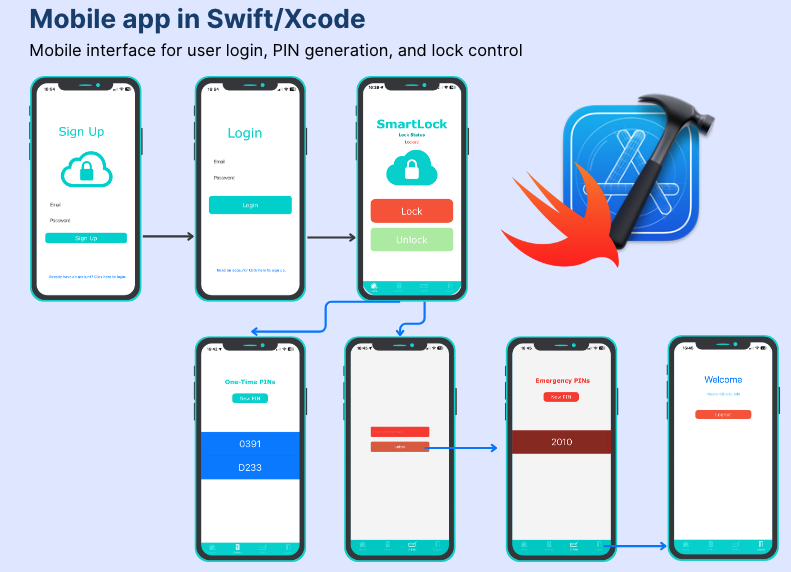
\includegraphics[width=1\textwidth]{img/softwareComponents.png}
    \label{fig:softwareComponents}
\end{figure}

\subsubsection{Cloud infrastructure}

Our current cloud infrastructure uses firestore database from firebase. Firebase was the easiest to use for our prototyping, and allowed us to quickly made the project functional. Though for the production system, we plan to use Amazon Web Services (AWS) along side Postgres so that we have more control on our database.  The current structure of our database only have a user controlling a lock, while we plan to update our cloud structure to have a many-to-many relationship. It should have a table for users and another table for locks, this way we can create a join table to join which users owns which lock and the lock is also able to know who the owner is. This is the common way people use the cloud structure to solve the many-to-many relationship.

\begin{figure}[!ht]
    \centering
    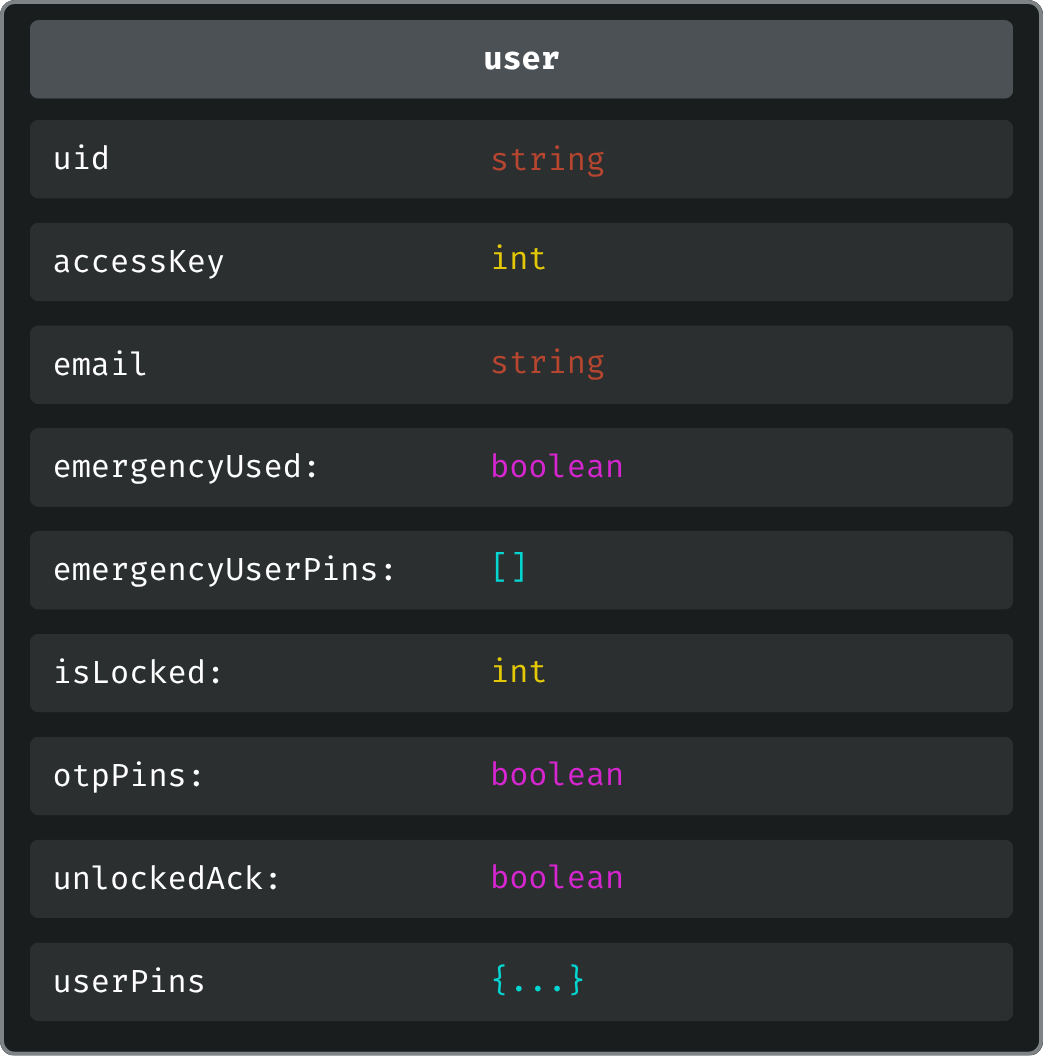
\includegraphics[width=1\textwidth]{img/db.png}
    \label{fig:firestoreSchema}
\end{figure}

\subsubsection{Results}

Our functional prototype was able to unlock and lock a door when asked to from the phone app. It can also generate pin codes that is for one time use, and the pin will be removed once the pin is used. Lastly we have an emergency pin that is used when the wifi is down. Once the emergency pin is used and the door lock is reconnected to wifi, it will remove the pin that is used. Compared to our manufactured product, we have a pin code to unlock the door but we did not have the feature of adding in how long the pin code lasts (having expiration on codes). As for the setup of the door lock, we used wifi provisioning instead of bluetooth since it seemed easier to create on ESP32-C3. Below we will have a figure of our final prototype and if you would like to see the demo of our prototype, the link is \href{https://youtu.be/XbD7zrFxasE?si=83Vg6o0KJSXbOtdF}{here}.

\begin{figure}[!ht]
\centering
\begin{subfigure}{.5\textwidth}
  \centering
  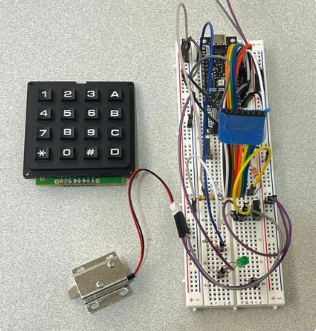
\includegraphics[width=.7\linewidth]{img/prototypeInside.png}
  \caption{inside of prototype}
  \label{fig:prototypeInside}
\end{subfigure}%
\begin{subfigure}{.5\textwidth}
  \centering
  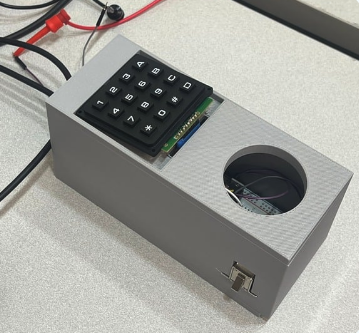
\includegraphics[width=.7\linewidth]{img/prototypeOutside.png}
  \caption{outside of prototype}
  \label{fig:prototypeOutside}
\end{subfigure}
\caption{Functional prototype result}
\label{fig:test}
\end{figure}

%% Testing Prototype %%

\subsection{Testing}
\subsubsection*{Firebase Mobile Connectivity Test}
\subparagraph{Test Goals and Purpose}
\begin{itemize}
    \item Ensure that an IOS device can securely connect and push data to the Firebase Firestore servers.
    \item What happens when there may be bad network connection
    \item Set a certain time frame for the pin to be qualified for
\end{itemize}

\subparagraph{Parameters}
\begin{itemize}
    \item 1/0 LOCK$\_$STATE necessary for defining lock-state, 1 is unlocked, 0 is locked.
    \item 7 digit QUALIFIED$\_$PIN list on an allow list for physical keypad on SmartLock.
    \item Make sure what data we send from phone is on firebase
    \item Provide time frame as input for start and expiration time for pin code
\end{itemize}

\subparagraph{Expectations of Test}
\begin{itemize}
    \item There will be no issue with pushing a simple piece of data for LOCK$\_$STATE to the firestore servers, clicking lock will properly push a 0 and clicking unlock will store a 1. Additionally, the pin list composed of generated and custom user pins will also have no trouble being communicated with Firestore servers to later be fetched by the physical device as an additional mechanism for locking and unlocking.
    \item Testing the time frame of the pin code, ensure only the time when valid to use the pin. Otherwise other times should be invalid.
\end{itemize}

\subsubsection{Lock Hardware Functionality Test}
\subparagraph{Test Goals and Purpose}
\begin{itemize}
    \item Ensure that an ESP32-C3 device can securely connect and retrieve data from the Firebase Firestore servers.
    \item Ensure that the ESP32-C3 board can correctly interact with hardware to enable mechanisms for locking/unlocking.
    \item Ensure that invalid codes should not release bolt, while valid codes should.
\end{itemize}


\subparagraph{Parameters}
\begin{itemize}
    \item 1/0 LOCK$\_$STATE necessary for defining lock-state, 0 is locked, 1 is unlocked. Retrieved from firebase.
    \item 7 digit QUALIFIED$\_$PIN list on an allow list for physical keypad on SmartLock.
\end{itemize}

\subparagraph{Expectations of Test}
\begin{itemize}
    \item The locking mechanism will respond appropriately after retrieving from Firestore, and the bolt will trigger when the parameter is set to 0 and likewise release given a 1 value. Additionally, the bolt will release given a valid input from the QUALIFIED$\_$PIN list and reject other non-valid input pins.
    \item Expecting the lock to not unlock after a code is expired, only unlock when it is still valid in a time frame.
\end{itemize}

\subsubsection{Multi-User \& Concurrency Test (Low Priority)}
\subparagraph{Test Goals and Purpose}
\begin{itemize}
    \item Ensure that multiple users can simultaneously interact with the smart lock through the mobile app and keypad without causing system conflicts.
    \item Verify that Firebase can handle concurrent updates to the lock state and PIN list without failure.
    \item Ensure the lock responds appropriately when multiple unlock requests are received from different users.
\end{itemize}


\subparagraph{Parameters}
\begin{itemize}
    \item Simultaneous requests from different mobile devices attempting to unlock/lock the door.
    \item Simultaneous PIN entries from different users on the physical keypad and mobile app.
\end{itemize}

\subparagraph{Expectations of Test}
\begin{itemize}
    \item Multiple users attempting to unlock the door at the same time should not cause conflicts or undefined behavior.
    \item The lock should process and execute the most recent valid request, ensuring no delays or duplicate actions.
    \item System logs should correctly track each user’s request, ensuring accountability and reliable data collection for user feedback.
\end{itemize}
\newpage

% New Section ----------------------------------------------------------------------------------------
\subsubsection{Administrative Details}

\subsubsection{Firebase Mobile Connectivity Test}
\textbf{\textit{Date $\&$ Location:}} Mar 12, 2025 in class
\newline
\textbf{\textit{Conducting Test:}} Jackson Kennedy, Adam Wu, Nathaniel Laurente, Neena Nguyen, and Professor Harrison.

\subsubsection{Lock Hardware Functionality Test}
\textbf{\textit{Date $\&$ Location:}} Mar 31, 2025 in class
\newline
\textbf{\textit{Conducting Test:}} Jackson Kennedy, Adam Wu, Nathaniel Laurente, Neena Nguyen, and Professor Harrison.

\subsubsection{Multi-User \& Concurrency Test}
\textbf{\textit{Date $\&$ Location:}} April 18, 2025 in class
\newline
\textbf{\textit{Conducting Test:}} Jackson Kennedy, Adam Wu, Nathaniel Laurente, Neena Nguyen, and Professor Harrison.

\subsubsection{Design of Experiment}
\subsubsection{Firebase Mobile Connectivity Test}
\textbf{\textit{Testing method type:}} Functional Testing, does the simple job of sending unlock or lock to firebase server, also sending pins.
\newline
\textbf{\textit{Test apparatus:}} Firebase Cloud service
\newline
\textbf{\textit{Independent Variables:}} Lock Status, Acceptable Pins
\newline
\textbf{\textit{Dependent Variables:}} N/A
\newline
\textbf{\textit{Number of factors:}}
\newline
\textbf{\textit{Sampling Procedures:}} 2 samples of observing Firestore for 1/0 LOCK$\_$STATE. 2 randomly generated PINs and 1 custom-user pin.

\subsubsection{Lock Hardware Functionality Test}
\textbf{\textit{Testing method type:}} When phone sends data for unlock or lock onto firebase, the lock should quickly retrieve information and respond accordingly. The purpose of this is to make sure the lock receives the data fast enough so that people waiting outside the lock does not wait too long for door to unlock. This should also be similar for the pin code case.
\newline
\textbf{\textit{Test apparatus:}} Utilize ESP32-C3 alongside a Solenoid door lock.
\newline
\textbf{\textit{Independent Variables:}} Make sure that the ESP32-C3 can read a simple "Hello world" on the server for basic testing.
\newline
\textbf{\textit{Dependent Variables:}} Everytime we are generating a new code from phone to firebase, the ESP32-C3 should also be able to retrieve those codes as valid codes immediately.
\newline
\textbf{\textit{Number of factors:}} N/A factors considered in this moment
\newline
\textbf{\textit{Sampling Procedures:}} Samples obtained from servers for LOCK\_STATE, only 0 or 1. Then we have samples for pin codes as well from Firebase.
\newline

\subsubsection{Multi-User \& Concurrency Test}
\textbf{\textit{Testing method type:}} Multiple phones will send an unlock signal from phone at nearly the exact same time and see if any undefined behavior occurs. Send a lock signal and an unlock signal at the same time to test if we can prioritize actions that came first, or lock the app after an action from one device has been made.
\newline
\textbf{\textit{Test apparatus:}} Mobile Device along with ESP32-C3.
\newline
\textbf{\textit{Independent Variables:}} Make sure that the ESP32-C3 can read a simple "Hello world" on the server for basic testing.
\newline
\textbf{\textit{Dependent Variables:}} ESP32-C3 behavior after multiple devices send a signal at the same time or immediately one after the other.
\newline
\textbf{\textit{Number of factors:}} 2 factors to be considered
\newline
\textbf{\textit{Sampling Procedures:}} Samples obtained from servers for LOCK\_STATE, only 0 or 1. Determine if multiple signals causes undefined or expected behavior.

\subsubsection{Testing Procedures}
\subsubsection{Safety Precautions}
Safety precautions for our project includes not having fast and forceful locks that can hurt individuals.

\subsubsection{Data Collection Method}
Collect data from the phone providing the custom pins onto firebase, as well as collecting data for locking or unlocking. We will also note down which users are grouped together to be able to use the same pin for unlcocking door.

\subsubsection{Observation of External Factors}
Some external factors that could make our product not function properly could include:

\begin{itemize}
    \item Bad network connection from phone or from ESP32-C3
    \item Firebase not loading properly
\end{itemize}

\subsection{Test Results}

\subsubsection{From Test Plan}
We will be testing our Firebase mobile connectivity, Esp32 hardware functionality, and multi-user and concurrency. For each of the tests, I will provide step by step instructions.

In the first test for Firebase mobile connectivity, we will test the connection between the mobile app and the firestore database. We will first build the mobile app and connect the firebase API keys to the app. Then with the mobile app, we will test the connection to the firestore database by sending a value to the database document. We can check if this succeeds by checking the firebase console and seeing if the value is updated.

In the second test for the ESP32 hardware functionality, we will test the connection between the ESP32 and wifi. Once connected to wifi, we will test the connection to the firestore database by using the API keys provided by firebase. Then we will create a document in the firestore database and use the ESP32 to fetch the document data. We can check if this succeeds by checking the fetched data is the same as the data in the firestore database. Also from the hardware functionality test, we are going to test the functionality of the solenoid lock, making sure that we can send a signal to unlock and lock the solenoid lock. One more test that we will need to take into consideration is the keypad functionality. We will test the functionality of the keypad by making sure that we can read the input from the keypad and send the input to the ESP32.

In the third test for multi-user and concurrency, we will test the connection between multiple mobile apps and the firestore database. We will first build the mobile app and connect the firebase API keys to the app. Then with the mobile app, we will test the connection to the firestore database by sending a value to the database document. We can check if this succeeds by checking the firebase console and seeing if the value is updated. We will then test the connection between multiple mobile apps and the firestore database by sending values to the database document from multiple mobile apps. We can check if this succeeds by checking the firebase console and seeing if the values are updated.

% GPT table
\subsubsection{Test Result Summary Table}
\begin{table}[h]
    \centering
    \resizebox{\textwidth}{!}{ % Resizes table to fit within page width
    \rowcolors{2}{teal!10}{teal!25}
    \begin{tabular}{|l|c|c|p{6cm}|}
        \hline
        \rowcolor{teal!50}
        \textbf{Objective ( Target )} & \textbf{Result} & \textbf{Met?} & \textbf{Discussion} \\
        \hline
        Firebase Connectivity & Appropriate 1/0 & N/A & Half this test done - explain how lock/unlock work but haven't tested PINs yet. \\
        
        Lock Hardware Functionality & N/A -\textit{Mar 31, 2025} & N/A & While this test has not been conducted yet, we suspect we will pass this test as the Firebase - Firestore lock/unlock was already successful, and the appropriate data was well-received by the ESP32-C3. All that remains is to ensure that the solenoid lock responds properly to an input signal, as well as compares and responds accordingly to valid/invalid codes. \\
        
        Concurrency & N/A -\textit{April 18, 2025} & N/A & While this test has not been conducted yet, we suspect that we will pass this test. Firebase should be able to handle multiple calls close to each other, as well as transmit this signal in the appropriate order. The Firestore database updated extremely quickly in real-time and shouldn't have trouble with concurrent calls. The PIN entries from different users also shouldn't cause conflict, and the door should unlock/lock as intended. \\
        
        \hline
    \end{tabular}}
\end{table}
